\documentclass{article}
\usepackage{amsmath}
\usepackage{tikz}
\usepackage{graphicx} % Required for inserting images

\title{Probability Theory Notes}
\author{Alex Gregory}
\date{July 2023}

\begin{document}

\maketitle

\section{Permutations}

Suppose we have a set of five characters $X = \{ A, B, C, D \}$. Suppose we select two characters at random from $X$ without replacement, how many possible combinations of characters are there?

For the first character, $c_1$, there are 4 possible outcomes: $A$, $B$, $C$, or $D$. For the second character, $c_2$, there are 3 possible outcomes depending on the $c_1$. Let us visualise these outcomes as a tree.

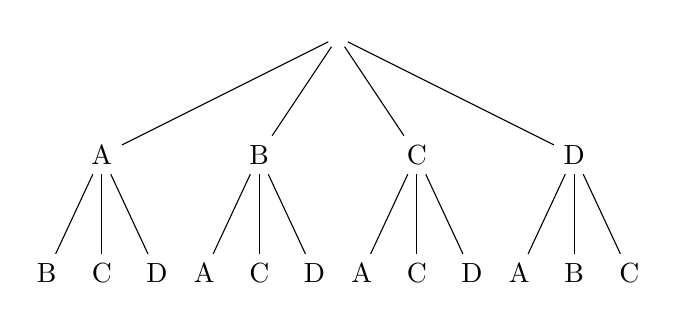
\begin{tikzpicture}
[
    level 1/.style = {sibling distance = 2cm},
    level 2/.style = {sibling distance = 0.7cm},
]
\node {} [sibling distance = 2.5cm]
    child {
        node {A}
        child {node {B}}
        child {node {C}}
        child {node {D}}
        edge from parent
    } 
    child {
        node {B}
        child {node {A}}
        child {node {C}}
        child {node {D}}
        edge from parent
    } 
    child {
        node {C}
        child {node {A}}
        child {node {C}}
        child {node {D}}
        edge from parent
    } 
    child {
        node {D}
        child {node {A}}
        child {node {B}}
        child {node {C}}
        edge from parent
    };
\end{tikzpicture}

From the tree above, it is clear there are $4 \cdot 3 = 12$ permutations. In general, if you have a game where there are $m$ steps and at each step, $i$, there are $n_i$ choices the total number of permutations is,
$$
    n_1 \times n_2 \times \dots \times n_m.
$$

\section{Combinations}

A combination is like a permutation but where the order is not important. So, where before we counted $AB$ as different to $BA$, now we treat them as the same.

Suppose again we have the set $X = \{ A, B, C, D \}$ and we select two characters at random without replacement. We know from the previous section there are $4 \cdot 3 = 12$ permutations of $X$. The possible permutations are as follows,
$$
\begin{matrix}
    AB & BA \\
    AC & CA \\
    AD & DA \\
    BC & CB \\
    BD & DB \\
    CD & DC \\
\end{matrix}
$$
Notice in the list of permutations each combination is repeated twice, for example $AB$ and $BA$. Therefore, if we divide the total number of permutations by the number of times each combination is repeated, we get the total number of combinations. For the example, this number of combinations is,
$$
\frac{4 \cdot 3}{2} = 6
$$
How do we find the number of times each combination is repeated in the list of permutations? Suppose for $X$ we want to know the number of times the combination $AB$ is repeated. $A$ can appear in the first or second position. Depending on the position of $A$, there is only one place where $B$ can be. So, the combination $AB$ is repeated, $2 \cdot 1 = 2$ times. The characters $AB$ are not important, in-fact any combination of characters is repeated $2$ times.

Suppose now that we select three characters from $X$ without replacement rather than two. The number of permutations is $4 \cdot 3 \cdot 2 = 24$. Consider the combination $ABC$. Again, again can be in the first, second or third position. Depending on the position of $A$, $B$ can be in two positions. Finally, depending on the position $A$ and $B$, $C$ must be in the remaining position. So each combination is repeated $3 \cdot 2 \cdot 1 = 6$ times. So, overall there are,
$$
    \frac{4 \cdot 3 \cdot 2}{3 \cdot 2 \cdot 1} = \frac{24}{6} = 4,
$$
combinations. The list of combinations are as follows,
$$
\begin{matrix}
    ABC \\    
    ABD \\
    BCD \\
    CAD \\
\end{matrix}
$$
Now consider the more general case. Suppose our set, $X$ has $n$ elements, and we want to find the number of combinations of length $r$ we can get from $X$. In English, the number of combinations is,
$$
\text{Number of combinations} = \frac{\text{Number of permutations}}{\text{Number of times each combination is repeated}}
$$
The number of permutations is $\frac{n!}{(n - r)!}$. The number of times each combination is repeated is $r!$. So, our formula becomes,
$$
\text{Number of combinations} = \frac{n!}{(n - r)!r!} = 
\begin{pmatrix} n \\ r \end{pmatrix}.
$$
The symbol $\begin{pmatrix}n \\ r\end{pmatrix}$ is referred to in English as $n$ choose $r$.

\subsection{Binomial Distribution}
Suppose we flip a coin 10 times. What is the probability we get $3$ heads? Naive guess might be 0.3 but we will see that is not the case.

We could get three heads in the first three tosses.
$$
    HHHTTTTTTT
$$
The probability of this event is $0.5 ^ {10}$. Equally, we could get the heads in the final three tosses.
$$
    TTTTTTTHHH
$$
The probability of this event is again $0.5 ^ {10}$. Since we are throwing a fair coin, the probability of any combination of ten heads and tails is $0.5 ^ {10}$. So, the probability of getting three heads is $0.5 ^ {10}$ multiplied by the number.

To count the number of combinations of three heads in ten tosses, we can use $n$ choose $r$ where $n$ is 10 and $r$ is three. The number of combinations is,
$$
    \begin{pmatrix}10 \\ 3\end{pmatrix} = \frac{10!}{7!3!} = \frac{720}{6} = 120
$$
Therefore, the probability of getting a three heads in ten tosses is,
$$
    120 \cdot 0.5 ^ {10} = 0.1171875
$$
Why do we count the number of combinations and not the number of permutations? First, label the heads of each coin toss as $X = \{ H_1, H_2, \dots, H_{10} \}$. The number of length three permutations for $X$ is,
$$
    10 \cdot 9 \cdot 8 = 720.
$$
However, this counts $\{ H_1, H_2, H_3 \}$ and $\{ H_2, H_1, H_3 \}$ as two separate outcomes. Counting these as two separate outcomes is not important to us as both mean the same thing i.e the first three tosses were heads.

In general, the formula for getting $i$ successes from $n$ trials is,
$$
    P(X = i) = \begin{pmatrix} n \\ i \end{pmatrix} p ^ {i} p ^ {n - i}.
$$
We also have a set of conditions such that a binomial distribution can be used:
\begin{itemize}
    \item The number of observations $n$ is fixed.
    \item The probability $p$ does not change during the experiment.
    \item The outcomes of each observation is either success or failure (heads or tails).
    \item Each observation is independent on one another.
\end{itemize}

\section{Poisson Distribution}

A random variable, $X$, that takes on values $0, 1, 2, \dots$ is said to follow the Poisson process if it has the following probability mass function
\begin{equation}
    P(X = i) = e ^ {-\lambda} \frac{\lambda ^ i}{i!}.
\end{equation}
For $i = 0, 1, 2, \dots$ and $\lambda > 0$. The Poisson distribution can approximate the binomial distribution with parameters $(n, p)$ if $n$ is large and $p$ is small. To see this suppose that $X$ is a random variable and let $\lambda = np$. Then,
\begin{align*}
    P(X = i) & = \frac{n!}{(n - i)!i!} p^i p^{n - i} \\
             & = \frac{n!}{(n - i)!i!} \left( \frac{\lambda}{n} \right)^i \left( 1 - \frac{\lambda}{n} \right)^{n - i} \\
             & = \frac{n(n-1)\dots(n-i+1)}{n^i} \frac{\lambda^i}{i!} \frac{(1 - \lambda / n)^n}{(1 - \lambda / n)^i}
\end{align*}
For large $n$ and moderate $\lambda$, we have
\begin{align*}
    \left(1 - \frac{\lambda}{n}\right)^n \approx e^{-\lambda}.
\end{align*}
The left most term approaches 1, and the denominator of the right most term approaches 1. Therefore,
\begin{equation*}
    P(X = i) = e^{-\lambda} \frac{\lambda^i}{i!}
\end{equation*}
So, if $n$ is large enough and $p$ is enough, the binomial distribution can be approximated with a Poisson distribution.

\subsection{Time Interval Poisson Distributions}

This section is taken from \cite{ross98}.

Suppose we have a random variable, $X$, that represents the number of successes that happen in an interval $t$. Such an event can be modelled with a Poisson distribution and in this section, we discuss how. This will only work if $\lambda$ satisfies the following assumptions:

\begin{itemize}
\item The probability that exactly one event occurs in the interval $h$ is $\lambda h + o(h)$ where $o(h)$ is any function, $f$ such that $\lim_{h \xrightarrow{} 0} f(h) / h = 0$
\item The probability that two of more events occur in $h$ is equal to $o(h)$.
\item For any integers $n, j_1, j_2, \dots, j_n$ and $n$ non-overlapping intervals, if we defined $E_i$ to be the even where exaction $j_i$ events occur in the $i$-th interval, then $E_1, E_2, \dots E_n$ are independent.
\end{itemize}
From these three assumptions, we can show that the number of events that happen at each interval of length $t$ can be modelled with a Poisson process.

Let the interval be $[0, t]$. Let $N(t)$ be the number of events that occur in the interval. We want to find the probability mass function $P(N(t) = k)$. First, we begin by breaking down the interval into non-overlapping sub-intervals of length $t / n$.

Let $P(N_1(t) = k)$ be the probability that $k$ sub-intervals have exactly one event happen in them. Let $P(N_2(t) = k)$ be the probability that one of the sub-intervals $N(t) = k$ and at least one of the sub-intervals has two or more events happen in it. Let us first show that $P(N_2(t) = k)$ tends to zero as $n$ approaches infinity.
\begin{align*}
    P(N_2(t) = k) & \leq P(\text{At least one sub-interval has 2 or more events}) \\
    & = P(\cup_{i=1}^{n} \text{$i$-th sub-interval has 2 or more events}) \\
    & \leq \sum_{i=1}^{n} P(\text{$i$-th sub-interval has 2 or more events})) \\
    & = \sum_{i=1}^{n} o(t / n) \\
    & = n \, o(t / n) \\
    & = t \frac{o(t / n)}{t / n} \\
\end{align*}
By our assumptions above, $o(t / n) / (t / n)$ tends to $0$ as $n$ approaches infinity. Therefore,
\begin{equation*}
    P(N_2(t) = k) \xrightarrow{n \rightarrow{} \infty} 0.
\end{equation*}
The first and second assumptions imply that the probability of getting $0$ events happen in a sub-interval is,
\begin{equation*}
    1 - \lambda h - o(h) - o(h) = 1 - \lambda h - o(h).
\end{equation*}
From the third assumption, $P(N_1(t) = k)$ is a binomial distribution. Therefore,
\begin{align*}
    P(N_1(t) = k) & =
    \begin{pmatrix} n \\ k \end{pmatrix}
    \left( \frac{\lambda t}{n} + o\left( \frac{t}{n} \right) \right) ^ k
    \left( 1 - \frac{\lambda t}{n} - o\left(\frac{t}{n}\right) \right) ^ {n - k} \\
    & =
    \begin{pmatrix} n \\ k \end{pmatrix}
    \frac{n}{n} \left( \frac{\lambda t}{n} + o\left( \frac{t}{n} \right) \right) ^ k
    \left( 1 - \frac{n}{n} (\frac{\lambda t}{n} - o\left(\frac{t}{n}\right))\right) ^ {n - k} \\
    & =
    \begin{pmatrix} n \\ k \end{pmatrix}
    \frac{1}{n} \left( \lambda t + t \frac{o(t / n)}{t / n} \right) ^ k
    \left( 1 - \frac{1}{n} (\lambda t - t\frac{o(t / n)}{t / n} ) \right) ^ {n - k} \\
\end{align*}
Since,
\begin{equation*}
    \frac{1}{n} \left( \lambda t + t \frac{o(t / n)}{t / n} \right) \xrightarrow{n \rightarrow \infty} \lambda t,
\end{equation*}
We get,
\begin{align*}
    P(N_1(t) = k) & =
    \begin{pmatrix} n \\ k \end{pmatrix}
    \left( \frac{\lambda t}{n} \right)^k
    \left( 1 - \frac{\lambda t}{n} \right) ^ {n - k} \\
    & =
    \begin{pmatrix} n \\ k \end{pmatrix}
    \left( \frac{\lambda t}{n} \right)^k
    \frac{(1 - \frac{\lambda t}{n})^n}{(1 - \frac{\lambda t}{n})^k} \\
    & =
    \frac{n(n - 1)\dots(n - k + 1)}{n^k}
    \frac{(\lambda t)^k}{k!}
    \frac{(1 - \frac{\lambda t}{n})^n}{(1 - \frac{\lambda t}{n})^k} \\
\end{align*}
The first term tends to 1 as $n$ approaches infinity. $(1 - \frac{\lambda t}{n})^n$ approaches $e^{-\lambda}$ and $(1 - \frac{\lambda t}{n})^k$ approaches 1 as $n$ approaches infinity. Therefore,
\begin{equation*}
    P(N(t) = k) = P(N_1(t) = k) = \frac{(\lambda t) ^ n}{n} e^{-\lambda}.
\end{equation*}
Therefore, this is a Poisson process.

\section{Distributions}

These notes follow \cite{ross98}.

\subsection{Uniform Distribution}

The uniform distribution is a distribution where every value equally likely. An example of a uniform distribution would be,
\begin{equation}
    f(x) =
    \begin{cases}
        1 \quad \text{if} \quad 0 < x < 1 \\
        0 \quad \text{Otherwise}
    \end{cases}
\end{equation}
The integral of this is, $\int_{-\infty}^{\infty} f(x) \, dx = 1 - 0 = 1$. If $0 < a <= b < 1$ the probability that $x$ is within $a$ and $b$ is,
\begin{equation*}
    f(a, b) = \int_{a}^{b} f(x) \, dx = b - a.
\end{equation*}
The general for of the uniform distribution on the range $0 < \alpha < \beta < 1$ is,
\begin{equation}
    f(x) =
    \begin{cases}
        \frac{1}{\beta - \alpha} \quad & \text{if} \quad \alpha < x < \beta \\
        0 \quad & \text{otherwise}
    \end{cases}
\end{equation}
This is a probability distribution since $\int_{-\infty}^{\infty} \frac{1}{\beta - \alpha} \, dx = \int_{\alpha}^{\beta} \frac{1}{\beta - \alpha} = \frac{\beta - \alpha}{\beta - \alpha} = 1$. The expected value and variance of the uniform distribution are,
\begin{align*}
    E(X) = & \int_{-\infty}^{\infty} x f(x) \, dx \\
         = & \int_{\alpha}^{\beta} \frac{x}{\beta - \alpha} \, dx \\
         = & \frac{x^2}{2(\beta - \alpha)} \Bigr|^{\beta}_{\alpha} \\
         = & \frac{\beta^2 - \alpha^2}{2(\beta - \alpha)} = \frac{(\beta - \alpha)(\beta + \alpha)}{2(\beta - \alpha)} = \frac{\beta + \alpha}{2}.
\end{align*}
So, the expected value is the midpoint $\alpha$ and $\beta$. To find the variance, we first need $E(X^2)$,
\begin{align*}
    E(X^2) = & \int_{-\infty}^{\infty} x^2 f(x) \, dx \\
           = & \int_{\beta}^{\alpha} \frac{x^2}{\beta - \alpha} \, dx \\
           = & \frac{x^3}{3(\beta - \alpha)} \Bigr|^{\beta}_{\alpha} \\
           = & \frac{\beta^3 - \alpha^3}{3(\beta - \alpha)} = \frac{\beta^2 + \alpha \beta + \alpha^2}{3}
\end{align*}
And so,
\begin{align}
    Var(X) = & E(X^2) - E(X)^2 \\ 
           = & \frac{\beta^2 + \alpha \beta + \alpha^2}{3} - \frac{\beta^2 + 2\alpha \beta + \alpha^2}{4} \\
           = & \frac{\beta^2 - 2\alpha\beta + \alpha^2}{12} \\
           = & \frac{(\alpha - \beta)^2}{12}
\end{align}

\subsubsection{Example}

Consider a random chord of a circle. What is the probability that the length of the chord will be greater than the side of the equilateral triangle inscribed in that circle?

First we need to know the length of the side of the equilateral triangle. Split the equilateral triangle into 3 smaller isoceles with with a point in the centre of the circle. Two of the sides in these isosceles triangles will have length of r. Split one of these triangles into two right angle triangles. One of the sides will have length r and one of the angles with be 60 degrees. Using trigonometry, the length of the opposite side is $r \sin \frac{\pi}{3}$.

Therefore, the length of one of the sides of the equilateral triangle is,
$$
    l = 2 r \sin \frac{\pi}{3}.
$$
A chord is formed when a straight line is drawn between two points on a circle. If we take two corners on the equilateral triangle join them at the centre of the circle, the angle will be 60 degrees. Let us call this length $l$. If we follow this same process with two random points, the chord, $m$, between them will be larger than $l$ if its angle is greater than $60$ degrees.

We need to know the probability this angle is greater than $60$ degrees.

If we pick a point at random and pick another point at random will be $\frac{1}{3}$.

\subsection{Exponential Distribution}

A random variable is said to have and exponential distribution if it has the following formula.
$$
    f(x) = 
    \begin{cases}
        \lambda e ^ {-\lambda x} \quad & \text{if} \, x \geq 0 \\
        0 \quad & \text{otherwise} \\
    \end{cases}
$$
We can find the mean and the variance from the moment generating function. This is calculated using integration by parts.
\begin{align}
    E(X^n) & = \int_{0}^{\infty} x^n \lambda e^{-\lambda x} \\
           & = - x^n e^{-\lambda x} \Bigr|^\infty_0 + \frac{n}{\lambda}\int_{0}^{\infty} x^{n - 1} e^{-\lambda x} \\
           & = 0 + \frac{n}{\lambda} E(X^{n - 1})
\end{align}
Therefore, the mean is,
\begin{equation}
    E(X) = \frac{1}{\lambda}.
\end{equation}
The second moment is,
\begin{equation}
    E(X) = \frac{2}{\lambda^2}.
\end{equation}
Thus, the variance is,
\begin{equation}
    Var(X) = E(X^2) - E(X)^2 = \frac{2}{\lambda^2} - \frac{1}{\lambda^2} = \frac{1}{\lambda^2}
\end{equation}
The exponential distribution is often used the model the time until and event happens. For example the time until a phone call ends.

\subsection{Gamma Distribution}

A random variable has a gamma distribution with $\lambda > 0$ and $\alpha > 0$ if its density is given by,
\begin{equation}
    f(x) =
    \begin{cases}
        \frac{\lambda e^{-\lambda x} (\lambda x)^{\alpha - 1}}{\Gamma(\alpha)} & x \geq 0 \\
        0 & x < 0
    \end{cases}
\end{equation}
Where $\Gamma(\alpha)$ is the gamma function, $\Gamma(\alpha) = \int_0^\infty e^{-y} y^{\alpha - 1} \, dy = (\alpha - 1)\Gamma(\alpha - 1)$.
\bibliography{bibliography}
\bibliographystyle{ieeetr}

\end{document}
